% !TEX encoding = UTF-8 Unicode
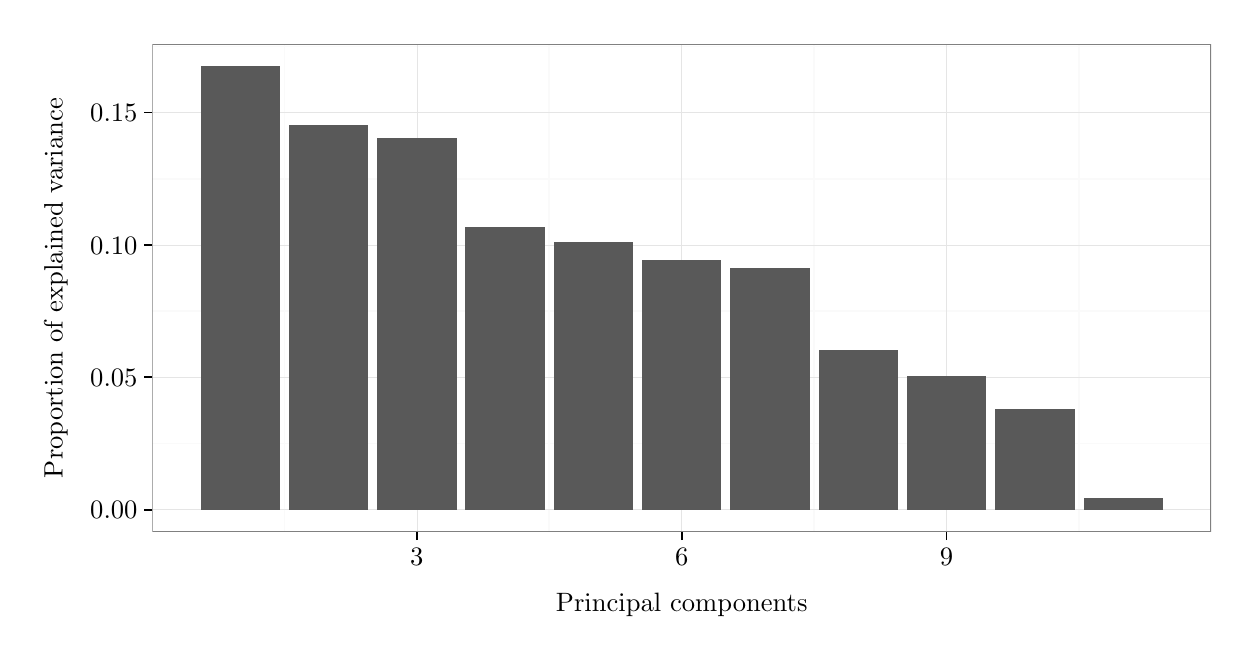
\begin{tikzpicture}[x=1pt,y=1pt]
\definecolor{fillColor}{RGB}{255,255,255}
\path[use as bounding box,fill=fillColor,fill opacity=0.00] (0,0) rectangle (433.62,216.81);
\begin{scope}
\path[clip] (  0.00,  0.00) rectangle (433.62,216.81);
\definecolor{drawColor}{RGB}{255,255,255}
\definecolor{fillColor}{RGB}{255,255,255}

\path[draw=drawColor,line width= 0.6pt,line join=round,line cap=round,fill=fillColor] (  0.00,  0.00) rectangle (433.62,216.81);
\end{scope}
\begin{scope}
\path[clip] ( 45.07, 34.62) rectangle (427.62,210.81);
\definecolor{fillColor}{RGB}{255,255,255}

\path[fill=fillColor] ( 45.07, 34.62) rectangle (427.62,210.81);
\definecolor{drawColor}{gray}{0.98}

\path[draw=drawColor,line width= 0.6pt,line join=round] ( 45.07, 66.54) --
	(427.62, 66.54);

\path[draw=drawColor,line width= 0.6pt,line join=round] ( 45.07,114.37) --
	(427.62,114.37);

\path[draw=drawColor,line width= 0.6pt,line join=round] ( 45.07,162.19) --
	(427.62,162.19);

\path[draw=drawColor,line width= 0.6pt,line join=round] ( 45.07,210.01) --
	(427.62,210.01);

\path[draw=drawColor,line width= 0.6pt,line join=round] ( 92.77, 34.62) --
	( 92.77,210.81);

\path[draw=drawColor,line width= 0.6pt,line join=round] (188.49, 34.62) --
	(188.49,210.81);

\path[draw=drawColor,line width= 0.6pt,line join=round] (284.21, 34.62) --
	(284.21,210.81);

\path[draw=drawColor,line width= 0.6pt,line join=round] (379.92, 34.62) --
	(379.92,210.81);
\definecolor{drawColor}{gray}{0.90}

\path[draw=drawColor,line width= 0.2pt,line join=round] ( 45.07, 42.63) --
	(427.62, 42.63);

\path[draw=drawColor,line width= 0.2pt,line join=round] ( 45.07, 90.46) --
	(427.62, 90.46);

\path[draw=drawColor,line width= 0.2pt,line join=round] ( 45.07,138.28) --
	(427.62,138.28);

\path[draw=drawColor,line width= 0.2pt,line join=round] ( 45.07,186.10) --
	(427.62,186.10);

\path[draw=drawColor,line width= 0.2pt,line join=round] (140.63, 34.62) --
	(140.63,210.81);

\path[draw=drawColor,line width= 0.2pt,line join=round] (236.35, 34.62) --
	(236.35,210.81);

\path[draw=drawColor,line width= 0.2pt,line join=round] (332.06, 34.62) --
	(332.06,210.81);
\definecolor{fillColor}{gray}{0.35}

\path[fill=fillColor] ( 62.46, 42.63) rectangle ( 91.18,202.80);

\path[fill=fillColor] ( 94.37, 42.63) rectangle (123.08,181.75);

\path[fill=fillColor] (126.27, 42.63) rectangle (154.99,176.77);

\path[fill=fillColor] (158.18, 42.63) rectangle (186.89,144.71);

\path[fill=fillColor] (190.08, 42.63) rectangle (218.80,139.32);

\path[fill=fillColor] (221.99, 42.63) rectangle (250.70,132.89);

\path[fill=fillColor] (253.90, 42.63) rectangle (282.61,129.93);

\path[fill=fillColor] (285.80, 42.63) rectangle (314.52,100.35);

\path[fill=fillColor] (317.71, 42.63) rectangle (346.42, 91.10);

\path[fill=fillColor] (349.61, 42.63) rectangle (378.33, 78.86);

\path[fill=fillColor] (381.52, 42.63) rectangle (410.23, 46.94);
\definecolor{drawColor}{gray}{0.50}

\path[draw=drawColor,line width= 0.6pt,line join=round,line cap=round] ( 45.07, 34.62) rectangle (427.62,210.81);
\end{scope}
\begin{scope}
\path[clip] (  0.00,  0.00) rectangle (433.62,216.81);
\definecolor{drawColor}{RGB}{0,0,0}

\node[text=drawColor,anchor=base east,inner sep=0pt, outer sep=0pt, scale=  0.96] at ( 39.67, 39.33) {0.00};

\node[text=drawColor,anchor=base east,inner sep=0pt, outer sep=0pt, scale=  0.96] at ( 39.67, 87.15) {0.05};

\node[text=drawColor,anchor=base east,inner sep=0pt, outer sep=0pt, scale=  0.96] at ( 39.67,134.97) {0.10};

\node[text=drawColor,anchor=base east,inner sep=0pt, outer sep=0pt, scale=  0.96] at ( 39.67,182.80) {0.15};
\end{scope}
\begin{scope}
\path[clip] (  0.00,  0.00) rectangle (433.62,216.81);
\definecolor{drawColor}{RGB}{0,0,0}

\path[draw=drawColor,line width= 0.6pt,line join=round] ( 42.07, 42.63) --
	( 45.07, 42.63);

\path[draw=drawColor,line width= 0.6pt,line join=round] ( 42.07, 90.46) --
	( 45.07, 90.46);

\path[draw=drawColor,line width= 0.6pt,line join=round] ( 42.07,138.28) --
	( 45.07,138.28);

\path[draw=drawColor,line width= 0.6pt,line join=round] ( 42.07,186.10) --
	( 45.07,186.10);
\end{scope}
\begin{scope}
\path[clip] (  0.00,  0.00) rectangle (433.62,216.81);
\definecolor{drawColor}{RGB}{0,0,0}

\path[draw=drawColor,line width= 0.6pt,line join=round] (140.63, 31.62) --
	(140.63, 34.62);

\path[draw=drawColor,line width= 0.6pt,line join=round] (236.35, 31.62) --
	(236.35, 34.62);

\path[draw=drawColor,line width= 0.6pt,line join=round] (332.06, 31.62) --
	(332.06, 34.62);
\end{scope}
\begin{scope}
\path[clip] (  0.00,  0.00) rectangle (433.62,216.81);
\definecolor{drawColor}{RGB}{0,0,0}

\node[text=drawColor,anchor=base,inner sep=0pt, outer sep=0pt, scale=  0.96] at (140.63, 22.61) {3};

\node[text=drawColor,anchor=base,inner sep=0pt, outer sep=0pt, scale=  0.96] at (236.35, 22.61) {6};

\node[text=drawColor,anchor=base,inner sep=0pt, outer sep=0pt, scale=  0.96] at (332.06, 22.61) {9};
\end{scope}
\begin{scope}
\path[clip] (  0.00,  0.00) rectangle (433.62,216.81);
\definecolor{drawColor}{RGB}{0,0,0}

\node[text=drawColor,anchor=base,inner sep=0pt, outer sep=0pt, scale=  0.96] at (236.35,  6.00) {Principal components};
\end{scope}
\begin{scope}
\path[clip] (  0.00,  0.00) rectangle (433.62,216.81);
\definecolor{drawColor}{RGB}{0,0,0}

\node[text=drawColor,rotate= 90.00,anchor=base,inner sep=0pt, outer sep=0pt, scale=  0.96] at ( 12.61,122.72) {Proportion of explained variance};
\end{scope}
\end{tikzpicture}
